\documentclass[11pt,a4paper]{article}

% ------------------------------------------------------------
% Pacotes (mesmo preâmbulo da proposta, report/report.tex)
% ------------------------------------------------------------
\usepackage[utf8]{inputenc}
\usepackage[T1]{fontenc}
\usepackage[brazil]{babel}
\usepackage{lmodern}
\usepackage{microtype}
\usepackage{amsmath,amssymb}
\usepackage{enumitem}
\usepackage{geometry}
\usepackage{titlesec}
\usepackage{booktabs}
\usepackage{graphicx}
\usepackage{caption}
\usepackage{hyperref}

% ------------------------------------------------------------
% Layout
% ------------------------------------------------------------
\geometry{top=1.8cm, bottom=1.8cm, left=1.9cm, right=1.9cm}

\setlength{\parindent}{0pt}
\setlength{\parskip}{3pt}
\setlist[itemize]{leftmargin=1.35em, itemsep=0.8pt, topsep=2pt, parsep=0pt}
\setlist[enumerate]{leftmargin=1.55em, itemsep=0.8pt, topsep=2pt, parsep=0pt}

\titleformat{\section}{\bfseries\normalsize}{}{0pt}{}
\titlespacing*{\section}{0pt}{7pt}{2pt}

\captionsetup{font=small, labelfont=bf, skip=3pt}
\setlength{\textfloatsep}{8pt}
\setlength{\floatsep}{6pt}

\hypersetup{colorlinks=true, linkcolor=black, urlcolor=blue}

\newcommand{\repo}{https://github.com/annwith/gender-representation-networks}
\newcommand{\dados}{\repo/tree/main/data/graphml}
\newcommand{\pagina}{https://annwith.github.io/gender-representation-networks/redes/}

% ------------------------------------------------------------
% Documento
% ------------------------------------------------------------
\begin{document}

\begin{center}
    {\large\bfseries MO438 -- Redes Complexas: Entrega Parcial (Visualização)}\\[2pt]
    Da rede lexical à rede contextual: reorganização das representações
    internas de Transformers com Redes Complexas\\[2pt]
    Juliana Midlej do Espirito Santo (RA 200208)
\end{center}

\vspace{-2mm}

% ============================================================
\section*{1. As redes}

Este arquivo traz a visualização (item 9) das quatro redes da entrega parcial. As redes têm os
mesmos 13.606 vértices: cada vértice é uma \textit{ocorrência} de um token em um parágrafo da
Wikipédia em português, de 8 temas. Cada ocorrência se liga às $k=10$ ocorrências de vetor
mais parecido (cosseno), e as redes diferem só no vetor: \textbf{lex}, o \textit{embedding} de
entrada do token no Qwen3-4B-Base (igual para todas as ocorrências do mesmo token), e
\textbf{L01}, \textbf{L18} e \textbf{L36}, a saída dos blocos 1, 18 e 36 do modelo. As figuras
mostram a versão não direcionada por união, com aresta $\{i,j\}$ quando $j$ está entre os
vizinhos de $i$ ou $i$ entre os de $j$; as arestas não têm peso. Sem o sentido dos arcos, a
versão direcionada tem exatamente as mesmas arestas, então as figuras valem para as duas
versões da entrega. A coleta dos dados, a construção das redes e as métricas dos itens 1 a 8
estão nos documentos da entrega parcial.

\textbf{Dados:} \url{\repo}; as redes, em GraphML, estão em
\href{\dados}{\texttt{data/graphml/}}. \textbf{Versão interativa}, com todos os vértices, busca
por palavra, a lista de vizinhos de cada ocorrência e outras cores (categoria do token, estrato
da amostra, comunidade): \url{\pagina}.

% ============================================================
\section*{2. Como as figuras foram feitas}

Cada rede tem o seu próprio layout, calculado pelo UMAP do \texttt{igraph}
(\texttt{layout\_umap}, sem pesos, \texttt{min\_dist} = 0,1, 500 épocas, semente 438). O UMAP
aproxima vértices ligados e afasta os não ligados. A distância no desenho só reflete a
estrutura da rede de forma aproximada, e a posição e a orientação absolutas não têm
significado: não dá para comparar posições entre os quatro desenhos. Cada painel mostra o
disco, centrado na posição mediana, que contém 99\% dos vértices; os 137 restantes de cada
rede, grupos pequenos empurrados para a periferia, ficam de fora (eles aparecem na versão
interativa). As arestas são traços finos e transparentes: onde há muitas, o fundo escurece. A
ordem em que os vértices são desenhados é sorteada, para que nenhuma cor fique sempre por cima.

A Fig.~\ref{fig:tema} colore os vértices pelo tema do artigo (o tema Esporte vem da categoria
Futebol). A Fig.~\ref{fig:palavra} usa os mesmos layouts e colore os vértices pela posição do
token na palavra: \emph{continua} quando a palavra segue no token seguinte (o token é o início
ou o meio de uma palavra de vários tokens), e \emph{termina} nos demais casos (último ou único
token da palavra, ou pontuação, que não pertence a nenhuma palavra). O \textit{tokenizer} separa
os números em dígitos, então todo dígito que não é o último do número também é
\emph{continua}. São 4.004 vértices \emph{continua} (29\% do total). As figuras e as
Tabelas~\ref{tab:arestas} e~\ref{tab:blocos} são geradas por
\texttt{scripts/partial\_delivery/draw\_networks.py}, a partir dos arquivos GraphML.

\begin{figure}[t]
\centering
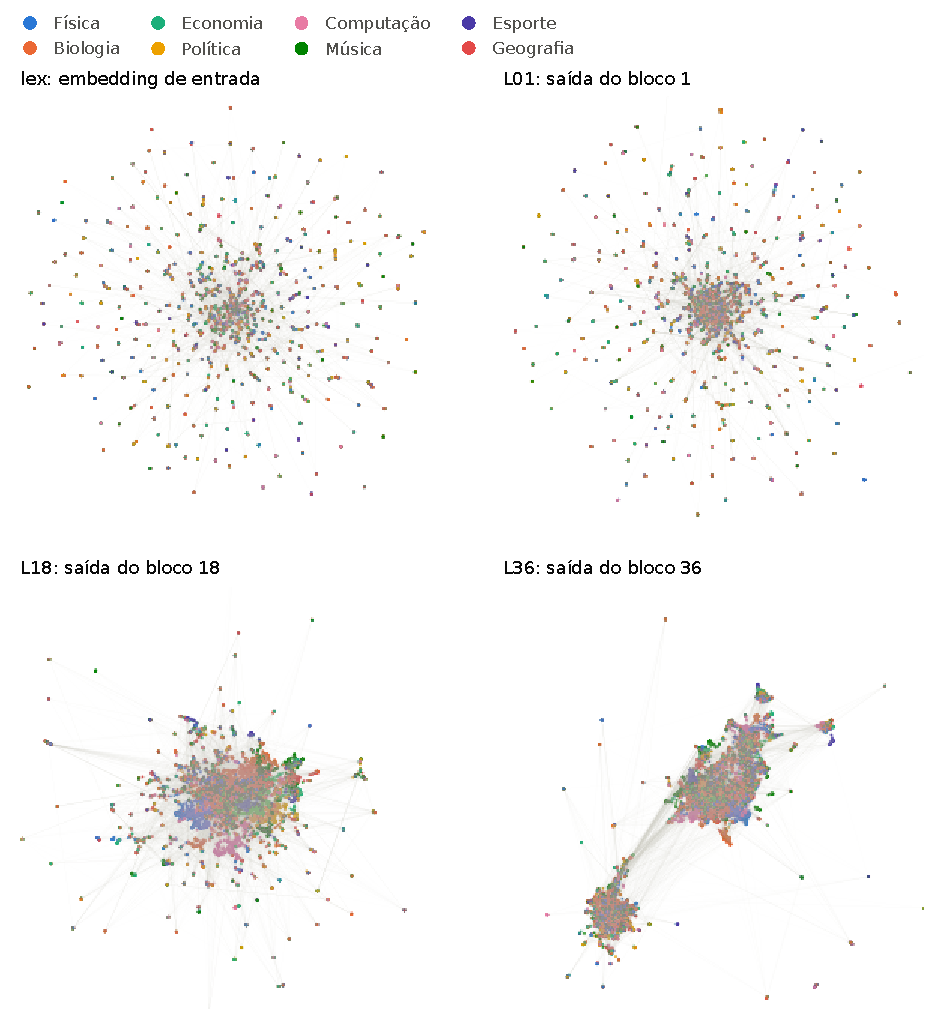
\includegraphics{figuras/redes.pdf}
\caption{As quatro redes, cada uma com o seu layout UMAP, com os vértices coloridos pelo tema
do artigo. Em cada painel ficam de fora os 137 vértices mais afastados do centro.}
\label{fig:tema}
\end{figure}

\begin{figure}[t]
\centering
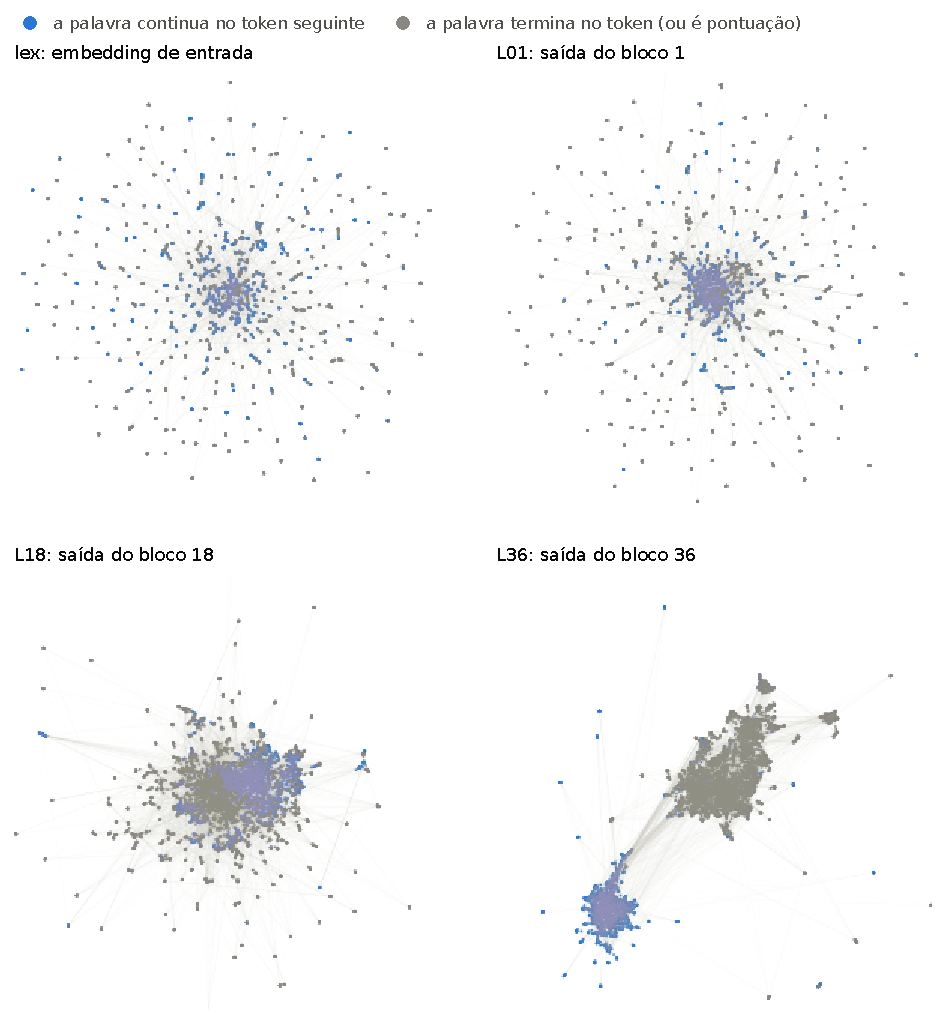
\includegraphics{figuras/redes_palavra.pdf}
\caption{Os mesmos desenhos da Fig.~\ref{fig:tema}, com os vértices coloridos pela posição do
token na palavra: em azul, as ocorrências em que a palavra continua no token seguinte
(\emph{continua}); em cinza, as demais (\emph{termina}).}
\label{fig:palavra}
\end{figure}

% ============================================================
\section*{3. O que as figuras mostram}

\begin{table}[h]
\centering
\small
\setlength{\tabcolsep}{3.5pt}
\caption{O que as arestas ligam nas quatro redes (união, $k=10$). As assortatividades são o
coeficiente de Newman para um atributo categórico: vale 1 quando toda aresta liga vértices da
mesma classe e 0 quando as arestas se distribuem entre as classes como ao acaso.}
\label{tab:arestas}
\begin{tabular}{lrrrr}
\toprule
Medida & lex & L01 & L18 & L36 \\
\midrule
Arestas entre ocorrências do mesmo token & 68,1\% & 63,6\% & 38,9\% & 20,8\% \\
Arestas entre ocorrências do mesmo tema & 20,4\% & 22,5\% & 52,4\% & 43,9\% \\
Assortatividade por tema & 0,087 & 0,111 & 0,454 & 0,357 \\
Arestas entre \emph{continua} e \emph{termina} & 14,6\% & 10,7\% & 10,4\% & 2,6\% \\
Assortatividade por posição na palavra & 0,621 & 0,741 & 0,749 & 0,938 \\
\bottomrule
\end{tabular}

\end{table}

\textbf{Por tema (Fig.~\ref{fig:tema}).} Em lex e L01, a rede se espalha em centenas de grupos
pequenos, em geral as ocorrências de um mesmo token, com temas misturados: em lex, 68\% das
arestas ligam ocorrências do mesmo token e só 20\% ligam ocorrências do mesmo tema
(Tabela~\ref{tab:arestas}). Em L18, os grupos se fundem num bloco central com regiões dominadas
por um tema: as arestas entre ocorrências do mesmo tema sobem para 52\%, e a assortatividade por
tema passa de 0,09 em lex para 0,45. Em L36, elas caem para 44\% (assortatividade 0,36), e a
rede se divide em dois blocos.

\textbf{Por posição na palavra (Fig.~\ref{fig:palavra}).} Em L36, o bloco menor é o das
posições em que a palavra continua no token seguinte. A separação aparece direto nas arestas
(Tabela~\ref{tab:arestas}): as arestas entre \emph{continua} e \emph{termina} são 10,4\% em L18
e só 2,6\% em L36, e a assortatividade por posição na palavra sobe de 0,75 para 0,94. Em lex
ela já é alta (0,62) porque ali a maioria das arestas liga ocorrências do mesmo token, e a
posição na palavra depende muito do token: um início de palavra, como \textit{Des}, sempre
continua. Em L36, onde só 21\% das arestas ligam ocorrências do mesmo token, a separação é a
maior das quatro redes.

\begin{table}[!htb]
\centering
\small
\setlength{\tabcolsep}{3.5pt}
\caption{Comunidades de Leiden (modularidade, melhor de 10 execuções) em resolução baixa,
$\gamma=0{,}05$, com o número de comunidades na resolução usual, $\gamma=1$, para comparação.
Blocos são as comunidades com ao menos 1\% dos vértices, e $B$ é o bloco com mais vértices
\emph{continua}.}
\label{tab:blocos}
\begin{tabular}{lrrrr}
\toprule
Medida & lex & L01 & L18 & L36 \\
\midrule
Comunidades com $\gamma = 1$ & 185 & 178 & 58 & 44 \\
Comunidades com $\gamma = 0{,}05$ & 113 & 121 & 9 & 5 \\
Blocos (comunidades com ao menos 1\% dos vértices) & 13 & 9 & 1 & 2 \\
\quad vértices nos blocos & 75,9\% & 75,7\% & 98,3\% & 98,8\% \\
\quad as duas maiores comunidades (vértices) & 6.338 / 670 & 7.850 / 505 & 13.381 / 51 & 9.431 / 4.012 \\
Bloco $B$ (vértices) & 6.338 & 7.850 & 13.381 & 4.012 \\
\quad fração de $B$ que é \emph{continua} & 40,1\% & 44,0\% & 29,8\% & 94,3\% \\
\quad fração dos \emph{continua} que está em $B$ & 63,5\% & 86,2\% & 99,5\% & 94,5\% \\
\quad arestas que saem de $B$ & 1,2\% & 1,0\% & 0,1\% & 1,0\% \\
\bottomrule
\end{tabular}

\end{table}

\textbf{Os dois blocos de L36.} Para delimitar os blocos sem depender do desenho, procuramos
comunidades com o algoritmo de Leiden numa resolução baixa (Tabela~\ref{tab:blocos}). Com
$\gamma=1$, ele divide cada rede em dezenas ou centenas de comunidades (de 44 em L36 a 185 em
lex); com $\gamma=0{,}05$, só separa grupos que quase não se ligam ao resto. Nessa resolução,
lex e L01 ainda se dividem em mais de cem comunidades, L18 fica num bloco só, com 98\% dos
vértices, e L36 se divide em dois blocos, de 9.431 e 4.012 vértices, que juntos reúnem 99\% dos
vértices. Só 1,0\% das arestas sai do bloco menor; 94,3\% dos seus vértices são
\emph{continua}, e ele reúne 94,5\% desses vértices. A última camada, que prepara a previsão do
próximo token, agrupa as ocorrências também pelo que deve vir depois, e não só pelo contexto
anterior.

\end{document}
